\documentclass[8pt]{scrartcl}
%\documentclass[8pt,landscape]{article}
\usepackage{multicol}
\usepackage{calc}
\usepackage{ifthen}
\usepackage[landscape]{geometry}
\usepackage{amsmath,amsthm,amsfonts,amssymb}
\usepackage{color,graphicx,overpic}
%\usepackage{hyperref}
\usepackage{enumitem}
\setlist{nolistsep}


\pdfinfo{
  /Title (EECS376ExamIStudyGuide.pdf)
  /Creator (TeX)
  /Producer (pdfTeX 1.40.0)
  /Author (Jason R. Berlinsky)
  /Keywords (pdflatex, latex,pdftex,tex)}

\ifthenelse{\lengthtest { \paperwidth = 11in}}
    { \geometry{top=.05in,left=.1in,right=.1in,bottom=.05in} }
    {\ifthenelse{ \lengthtest{ \paperwidth = 297mm}}
        {\geometry{top=1cm,left=1cm,right=1cm,bottom=1cm} }
        {\geometry{top=0.25cm,left=0.25cm,right=0.25cm,bottom=0.51cm} }
    }

\pagestyle{empty}

\makeatletter
\renewcommand{\section}{\@startsection{section}{1}{0mm}
                                {-1ex plus -.5ex minus -.2ex}
                                {0.5ex plus .2ex}
                                {\normalfont\large\bfseries}}
\renewcommand{\subsection}{\@startsection{subsection}{2}{0mm}
                                {-1explus -.5ex minus -.2ex}
                                {0.5ex plus .2ex}
                                {\normalfont\normalsize\bfseries}}
\renewcommand{\subsubsection}{\@startsection{subsubsection}{3}{0mm}
                                {-1ex plus -.5ex minus -.2ex}
                                {1ex plus .2ex}
                                {\normalfont\small\bfseries}}
\makeatother

\def\BibTeX{{\rm B\kern-.05em{\sc i\kern-.025em b}\kern-.08em
    T\kern-.1667em\lower.7ex\hbox{E}\kern-.125emX}}

\setcounter{secnumdepth}{0}


\setlength{\parindent}{0pt}
\setlength{\parskip}{0pt plus 0.01ex}

\newtheorem{example}[section]{Example}
% -----------------------------------------------------------------------

\begin{document}

\raggedright
\footnotesize
\begin{multicols}{6}


% multicol parameters
% These lengths are set only within the two main columns
%\setlength{\columnseprule}{0.25pt}
\setlength{\premulticols}{1pt}
\setlength{\postmulticols}{1pt}
\setlength{\multicolsep}{1pt}
\setlength{\columnsep}{1pt}

%\begin{center}
%     \Large{\underline{Title}} \\
%\end{center}

\section{Equivalence Relations}
$R$ is {\bf reflexive} if for every $x$, $xRx$\\
$R$ is {\bf symmetric} if for every $x$ and $y$, $xRy$ implies $yRx$\\
$R$ is {\bf transitive} if for every $x, y, z$, $xRy \wedge yRz \rightarrow xRz$
\section{Boolean Logic}
$\neg$ - Not\\
$\wedge$ - And\\
$\vee$ - Or\\
$P \wedge (Q \vee R) = (P \wedge Q) \vee (P \wedge R)$\\
$P \vee (Q \wedge R) = (P \vee Q) \wedge (P \vee R)$\\
For any two sets $A$ and $B$, $\bar{A \cup B} = \bar{A} \cap \bar{B}$
\section{Finite Automata}

\subsection{DFA}

\begin{multicols}{2}

Each state must have exactly one transition arrow for every item in the alphabet, and it may only occupy a single state at a time. Formally described by $(Q, \Sigma, \delta, q_0, F)$, where $Q$ is a finite set of states (as $\{q_0, q_1, q_2\}$), $\Sigma$ is the alphabet, $\delta$ is the transition function with domain $Q x \Sigma$ and range $Q$ ($Q x \Sigma \rightarrow Q$), $q_0$ is the start state $\in Q$, and $F$ is the set of accept states, which may be the empty set, $\subset Q$.

\begin{center}
    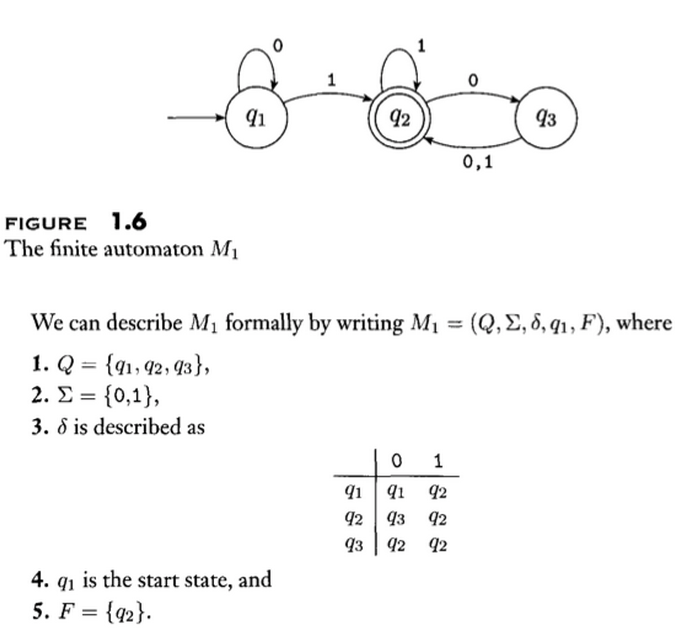
\includegraphics[scale=0.25]{dfa_sample.png}
\end{center}

\end{multicols}

\subsubsection{Complementation}

Flip acceptance states to get the complement.

\subsubsection{Combining}

Let's say there are two DFAs, $A = (Q_1, \Sigma, \delta_1, q_1, F_1)$ and $B = (Q_2, \Sigma, \delta_2, q_2, F_2)$. Let the intersection of the two, $C = (Q_1 \times Q_2, \Sigma, \delta_3, (q_1, q_2), F_1 \times F_2)$, where $\delta_3((r_1, r_2), a) = (\delta_1(r_1, a), \delta_2(r_2, a))$. The union of the two is given by closure properties:
$A \cup B = \overline{\bar{A} \cap \bar{B}}. F_3 = \overline{\bar{F_1} \times \bar{F_2}}$ 

\subsection{Regular Operations}

Union ($\cup$): Returns a set containing all elements that appear in either set.\\
Concatenation ($.$): Returns a set containing all combinations of an element from set $A$ and an element from set $B$\\
Star ($*$): Returns a set containing all permutations of each element in a given language. This returns an infinite set. Also all words over the alphabet.

%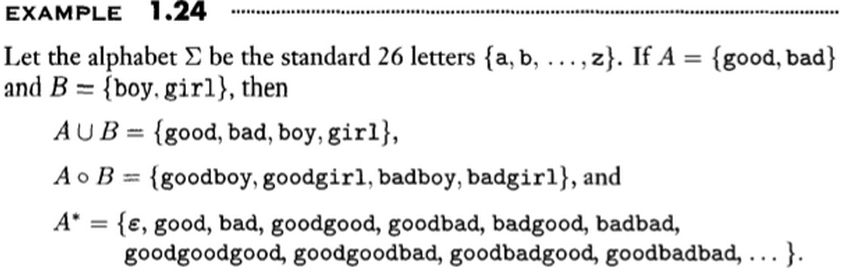
\includegraphics[scale=0.35]{operations.png}

\subsection{Non-Deterministic}

A more generalized form of a DFA. Each state does not need a transition arrow for each element in the alphabet. May have more than one active state, may also have more than one transition arrow for a given element in the alphabet. Have a special symbol $\epsilon$ which is followed when present as a transition and does not ``eat" a character from the string.

Try all legal transitions in parallel. On choice, pick/guess best transition towards acceptance. Accept if there is some path from start to accept.

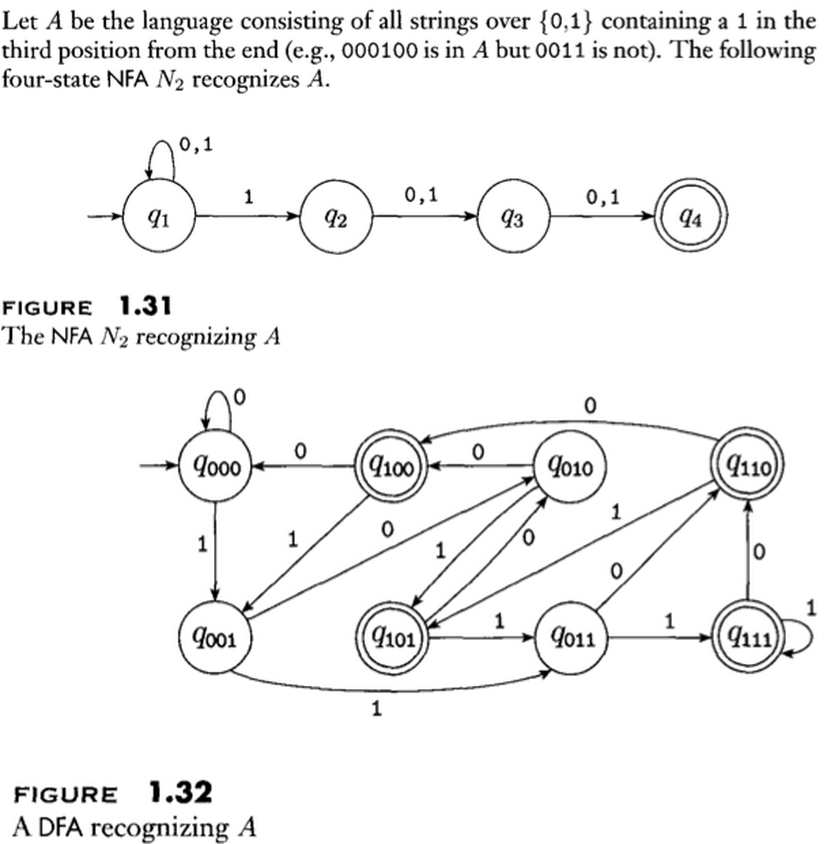
\includegraphics[scale=0.25]{nfa_dfa.png}

\section{Closure and Projection}

{\bf Closure:} The idea that any of the regular operations performed on two regular languages will result in another regular language.

{\bf Projection:} The intersection where all elements in both sets will be present in the new set.

\section{Regular Expressions}

Formal definition ($R_n$ are regexps):
\begin{multicols}{2}
\begin{itemize}
    \item $\alpha$ for some $a$ in the alphabet $\Sigma$
    \item $\epsilon$
    \item $\emptyset$
    \item $(R_1 \cup R_2)$
    \item $(R_1 . R_2)$
    \item $(R_1^*)$
\end{itemize}
\end{multicols}

$\alpha$ and $\epsilon$ represent the languages $\{\alpha\}, \{\epsilon\}$ respectively, and $\emptyset$ is the empty language. The remaining show what happens when a closure property is applied on the base languages.

Symbols:
\begin{itemize}
    \item $\Sigma$: Any symbol in the alphabet
    \item $*$: Repeat the previous character $0$ or more times
    \item $+$: Repeat the previous character $1$ or more times.
\end{itemize}
Definitions:
\begin{multicols}{2}
\begin{itemize}
    \item $R \cup \emptyset = R$ - Adding the empty language to any other language will not change it
    \item $R . \epsilon = R$ - Joining the empty string to any other string is the same string
    \item $A^* = \{\epsilon\} \cup A \cup AA \cup AAA \cup ...$
    \item $|A \cup B| <= |A| + |B|$
    \item $|AB| <= |A| . |A|$
    \item $\emptyset^* = \{\epsilon\}$. If $A \neq \emptyset$, then $A^*$ is infinite
    \item $L(\underline{\emptyset}) = \emptyset$
    \item $L(\underline{\epsilon}) = \{\epsilon\}$
    \item $L((a \cup b)\epsilon) = \{a, b\}$
    \item $L((a \cup b)\emptyset) = \emptyset$
\end{itemize}
\end{multicols}

\subsection{NFA $\rightarrow$ DFA}

Given a set $R \subseteq Q$ of states in $A_1$, let $E(R)$ be the states reachable from $R$ by following $0$ or more $\epsilon$-transitions. Given NFA $A_1 = (Q, \Sigma, \delta, q_0, F)$, construct DFA $A_2 = (Q', \Sigma', \delta', q_0', F')$. $Q' = P(Q)$, $q_0' = E(\{q_0\})$ (states reachable from $q_0$ by $\epsilon$-archs. For $R \in Q'$ and $a \in \Sigma$, let $\delta'(R, a) = \{q \in Q | \exists r \in R q \in E(\delta(r, a))\}$ (states reachable from some $r \in R$ by an $a$ arc followed by any number of $\epsilon$ arcs. $F' = \{R \in Q' | R$ contains an accept state of $A_1\}$

\subsection{Regex $\rightarrow$ NFA}

\begin{center}
    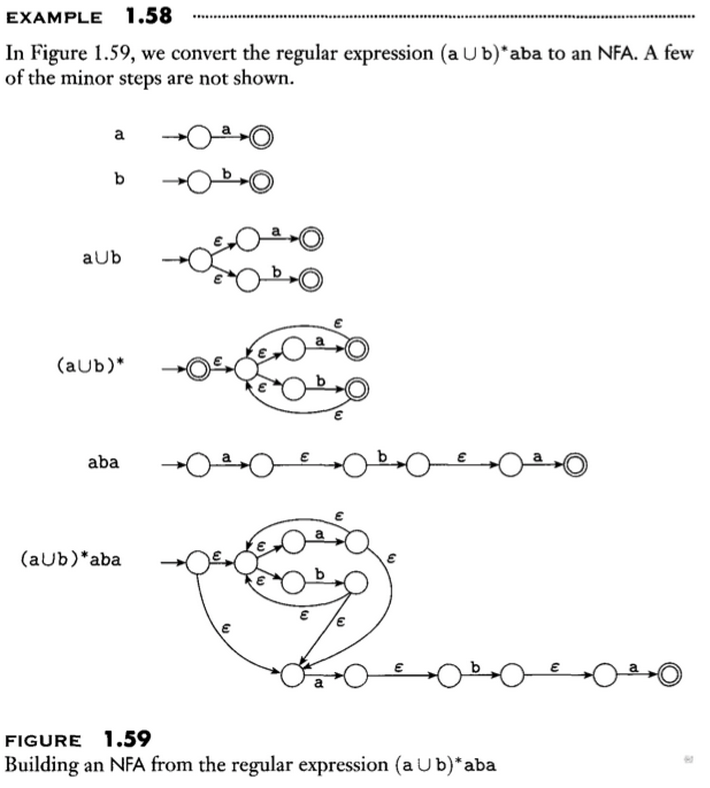
\includegraphics[scale=0.25]{regex_to_nfa.png}
\end{center}

\subsection{NFA $\rightarrow$ Regex}

Remove states one at a time, maintain equivalence, until we get two states with one regex transition.
\begin{itemize}
    \item Add new start state with an $\epsilon$ arc to old start state
    \item Add new single ccpet state, connected with $\epsilon$ arcs from old accept states
    \item No arcs into start state or out of accept state
    \item All other arcs present (with $\emptyset$ label if necessary)
\end{itemize}


\subsection{DFA $\rightarrow$ Regex}

This is aided by a {\bf generalized nondeterministic finite automaton} defined as the 5-tuple $(Q, \Sigma, \delta, q_{start}, q_{accept})$. $Q$ is the finite set of states, $\Sigma$ is the input alphabet, $delta: (Q - \{q_{accept}\}) x (Q - \{q_{start}\}) \rightarrow R$ is the transition function.

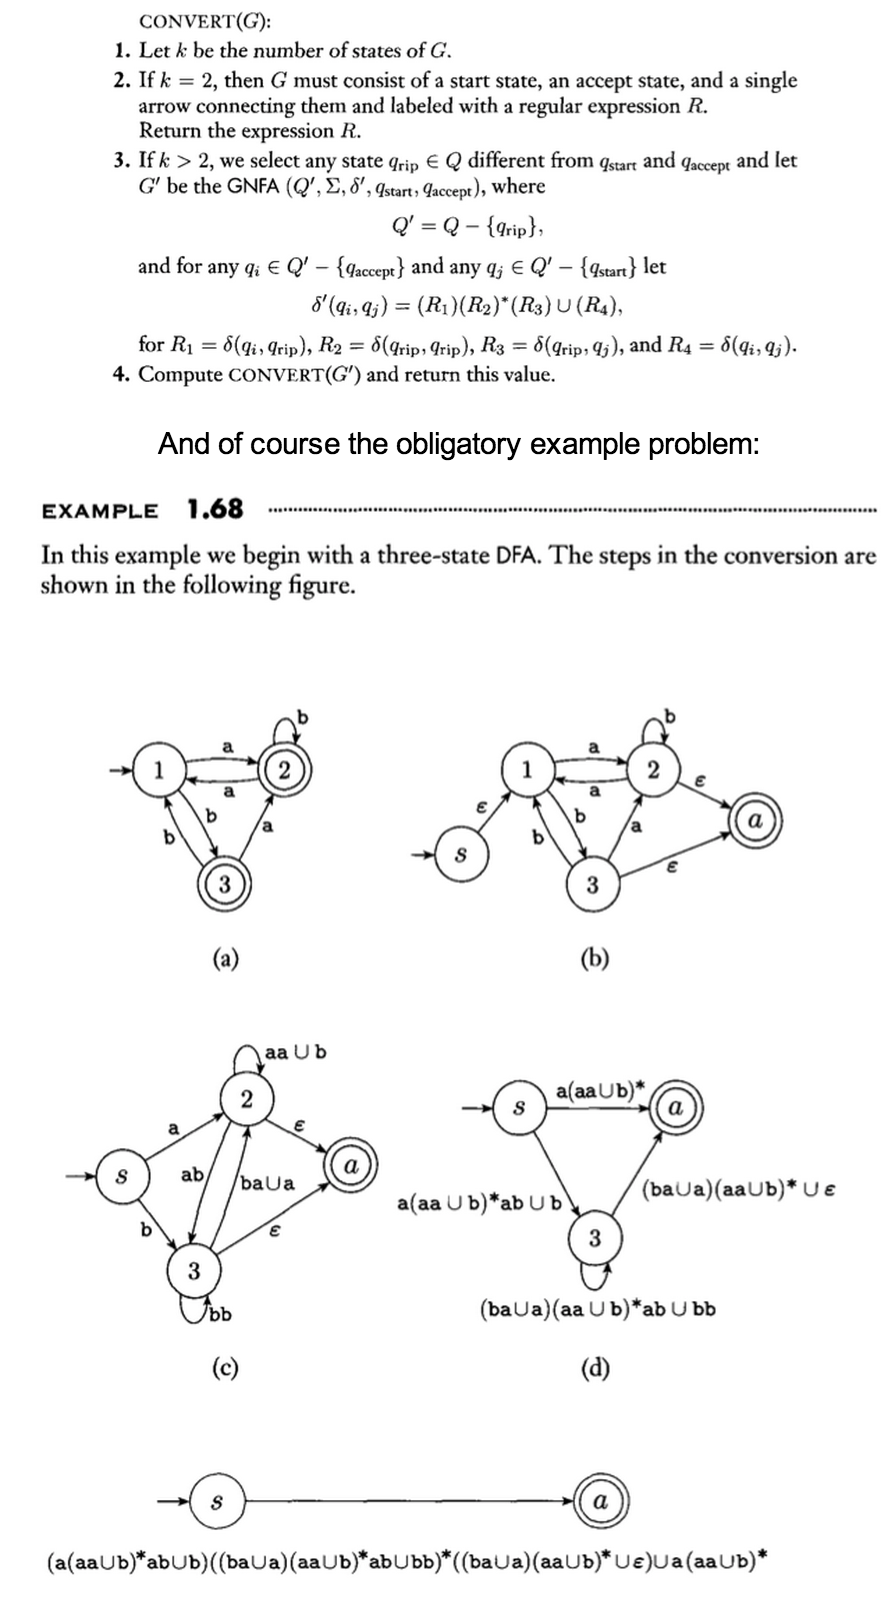
\includegraphics[scale=0.25]{dfa_to_regex.png}

\section{Nonregular Languages}

Any language that can not be determined in a finite amount of states on a DFA or NFA is nonregular. Good examples are languages that require the knowledge of a previous count to prove them, such as a language that has some number of $0$ followed by the same number of $1$s.

\subsection{Pumping Lemma}

The pumping lemma is a simple proof to show that a language is not regular, meaning a FSM can not be built for it. The canonical example is the language $(a^n)(b^n)$. It is trivial to build a FSM for some examples:

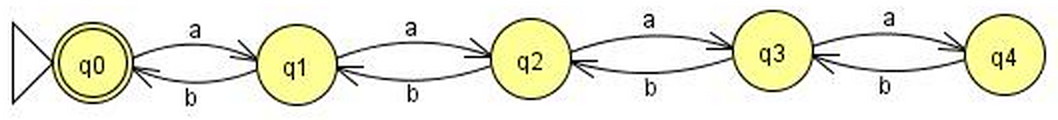
\includegraphics[scale=0.25]{simple_pumping_fsm.png}

Such an FSM will work all the way up to $n = 4$, but the language does not constrain $n$. No matter how many states are added to the FSM, there will be an input where $n$ is the number of states plus $1$, and the machine will fail. Therefore, we must add a loop in the FSM to keep the number of states finite, as such:

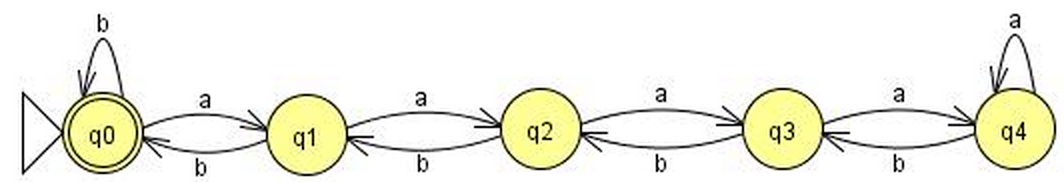
\includegraphics[scale=0.25]{loop_pumping_fsm.png}

This will work. However, after the first $4$ $a$s, the machine loses count of how many have bene input because it stays in the same state. Therefore, this erroneously accepts the string $aaaa(a^*)bbbb$. We can say that $(a^*)$ can be pumped. The fact that the FSM is finite and $n$ is not bounded guarantees that any machine which accepts all strings in the language must have this property -- the machine must loop at some point, and when it loops, the language can be pumped. Therefore, no FSM can be built for this language, thus it is not regular.

Mathematically, let $L$ be a regular language. Then there exists an integer $p >= 1$ depending only on $L$ such that every string $w$ in $L$ of length $>= p$ can be written as $w = wyx$, i.e. $w$ can be divided into 3 substrings, such that:

\begin{itemize}
    \item $|y| >= 1$
    \item $xy <= p$
    \item $\forall i >= 0, xy^iz \in L$
\end{itemize}

$y$ is the substring that can be {\bf pumped} (removed or repeated any number of times, and the resulting string is always in $L$). $(1)$ means the loop $y$ to be pumped must be of length at least $1$, $(2)$ means the loop must occur within the first $p$ characters. $|x|$ must be smaller than $p$ by $(1)$ and $(2)$; apart from that there is no restriction on $x$ and $z$.

In other words, for any regular language $L$, any sufficiently long word $w \in L$ can be split into $3$ parts, $w = xyz$, such that all the strings $xy^kz$ for $k >= 0$ are also in $L$.

\subsubsection{Game}

Consider $ADD = \{$``$a + b = c$"$\}$, e.g. $2 + 3 = 5 \in ADD$, but $2 + 3 = 6 \notin ADD$.

Can a $17$-state DFA $M$ recognize this language? {\bf No}. Consider $1, 2, 3, ..., 18$ as the value for $a$. Two different numbers, e.g. $2$ and $5$, get $M$ to the same state. Then $2 + 1 = 3, 5 + 1 = 3$ take $M$ to the same state. {\bf CONTRADICTION}.

Paula wants to prove that a language is regular; skeptical Victor wants to verify.

Paula: ``This 17-state $M$ recognizes $ADD$\\
Victor: ``Oh, really? What if we start with $1, 2, ..., 18$?\\
{\bf Victor wins; $ADD$ is not regular}

\hline

Show $A = \{ww: w \in \Sigma^*\}$ is not regular.

Paula: $p$\\
Victor: $w = 10^{p+1}$\\
Paula: $ww = xyz$ with $|y| > 0, |xy| <= p$\\
Victor: $i = 0$\\
$y \in 0^+$ has exactly one $1$. $x = $``1", $y =$ ``00", $z =$ ``0010000" $\rightarrow w =$ ``1000010000". Alternatively, $w = 1000|010|000$. So $xz$ has unequal $0$ fields or an odd number of $1$s. $xz \notin A \rightarrow$ contradiction.

\subsubsection{General for Regular Languages}

If a language $L$ is regular, then there exists a number $p >= 1$ such that every string $uwv \in L$ with $|w| >= p$ can be written in the form $uwv = wxyzv$ with strings $x, y, z$ such that $|xy| <= p, |y| >= 1$, and $uxy^izv \in L \forall i >= 0$.

\subsubsection{Converse}

The converse of the pumping lemma is not true; a language that satisfies the conditions may still be non-regular. Both the original and general versions of the lemma necessary {\bf but not sufficient condition} for the language to be regular.

\section{Turing Machines}

Hypothetical devices that manipulate symbols on a strop of tape according to some table of rules. Consists of:

\begin{itemize}
    \item A {\bf tape} divided into cells, one next to the other. Each cell contains a symbol from some finite alphabet. The alphabet contains some special blank symbol and one or more other symbols. The tape is assumed to be arbitrarily extendable to the left and right. Cells that have no content are assumed to be filled with the blank symbol.
    \item A {\bf head} that can read and write symbols on the tape and move the tape left and right one cell at a time.
    \item An {\bf action table or transition function} of instructions that, given the state the machine is currently in and the current symbol being read from the tape, tells the machine to do the folliwing in sequence:
    
    \begin{itemize}
        \item Either erase or write a symbol, and then
        \item Move the head, and then
        \item Assume the same or a new state as prescribed
    \end{itemize}
\end{itemize}

Note that every part of the machine and its actions is finite, discrete and distinguishable.

\subsection{Formal Definition}

7-tuple $M = (Q, \Gamma, \beta, \Sigma, \delta, q_0, F)$, where:

\begin{itemize}
    \item $Q$ is a finite, non-empty set of states
    \item $\Gamma$ is a finite, non-empty set of the tape alphabet/symbols
    \item $\beta \in \Gamma$ is the blank symbol (the only symbol allowed to occur on the table indefinitely often at any step during the computation)
    \item $\Sigma \subseteq (\Gamma - \{\beta\})$ is the set of input symbols
    \item $q_0 \in Q$ is the initial state
    \item $F \subseteq Q$ is the set of final/accepting states
    \item $\delta: (Q - \{F x \Gamma\}) \rightarrow Q x \Gamma x \{L, R\}$ is a partial function called the transition function, where $L$ is left shift, $R$ is right shift, $N$ is no shift.
\end{itemize}

\subsubsection{3-State Busy Beaver}

A turing machine that attains the maximum number of steps performed or number of nonblank symbols finally on the tape among all Turing machines of a certain class.

\begin{itemize}
    \item $Q = \{A, B, C, HALT\}$
    \item $\Gamma = \{0, 1\}$
    \item $\beta = 0$ ("blank")
    \item $\Sigma = \{1\}$
    \item $q_0 = A$ (initial state)
    \item $F = \{HALT\}$
    \item $\delta$ is given on attached page
\end{itemize}

\section{Decidable Languages}

A decidable language is:

\begin{itemize}
    \item A recursive subset in the set of all possible words over the alphabet of the language
    \item A formal language for which there exists a Turing machine which will, when presented with any finite input string, halt and accept if the string is in the language, and halt and reject otherwise. The Turing machine always halts; it is known as a decider and is said to decide the language.
\end{itemize}

\subsection{Decider}

A decider is a machine that halts for every input. Also known as a total turing machine. $L(M)$ is decidable.

\subsection{Closure Properties}

Decidable languages are closed under the following operations (if $L$ and $P$ are two decidable languages, then the following are also decidable):

\begin{itemize}
    \item Kleene star $L^*$
    \item Concatenation $L . P$
    \item Union $L \cup P$
    \item Intersection $L \cap P$
    \item Complement $\bar{L}$
    \item Set difference $L - P$ (can be expressed in terms of intersection and complement)
\end{itemize}

\subsection{Decidability}

Let $A_{DFA} = \{<B, w> | B$ is a DFA that accepts input string $w \}$

\begin{itemize}
    \item Need to present a Turing machine $M$ that decides $A_{DFA}$
    \item $M = $``On input $<B, w>$, where $B$ is a DFA and $w$ is a string:
    \begin{itemize}
        \item Simulate $B$ on input $w$
        \item If the simulation ends in an accept state, accept. Otherwise, reject
    \end{itemize}
    \item When $M$ receives its input, it checks whether the input is actually a DFA and string. If not, reject.
    \item $M$ then carries out the simulation, keeping track of $B$'s state and position on its tape
    \item When $M$ finishes processing the last symbol of $w$, it accepts if $B$ is in an accepting state; rejects otherwise.
\end{itemize}

\subsection{Undecidable Languages}

Assume that $A_{TM} = \{<M, w>: M(w)$ enters ``accept"$\}$ is undecidable. The following are undecidable:
\begin{itemize}
    \item $\{<M, w>: M(w)$ enters state $q_5\}$
    \item $\{<M, w>: M(w)$ prints $5\}$
    \item $\{<M, w>: M(w)$ enumerates $0^n1^n\}$
    \item $\{<M>: M()$ enumerates $0^n1^n\}$
    \item $\{<M>: M()$ enumerates a regular language$\}$
    \item $\{<M>:$ For $M$ as an enumerator, $L(M)$ is regular$\}$
    \item $\{<M>:$ For $M$ as a recognizer, $L(M)$ is regular$\}$
    \item $\{<M>:$ For $M$ as a recognizer, $L(M)$ is ...$\}$
\end{itemize}

\subsubsection{Halting Problem}

$A_{TM} = \{<M, w> | M$ is a TM and $M$ accepts $w\}$\\
Theorem: $A_{TM}$ is undecidable.\\
Proof:

\begin{itemize}
    \item Assume $A_{TM}$ is decidable. Suppose $H$ is a decider for $A_{TM}$: $H(<M, w>) = \{$accept if $M$ accepts $w$; reject otherwise$\}$
    \item Construct a new TM $D$ that calls $H$ to determine what $M$ does when $M$ is its own input. $D = $``On input $<M>$:
    \begin{itemize}
        \item Run $H$ on input $<M, <M> >$
        \item Output the opposite of what $H$ outputs
    \end{itemize}
    \item Example of $D$: $D(<M>) = \{$ accept if $M$ does not accept $<M>$, reject if $M$ accepts $<M>\}$
    \item Run $D$ with itself as input: $D(<D>) = \{ $accept if $D$ does not accept $<D>$; reject if $D$ accepts $<D>\}$
    \item No matter what $D$ does, it is forced to do the opposite $\rightarrow$ contradiction. Thus, neither $D$ nor $H$ can exist. Therefore, $A_{TM}$ is undecidable.
\end{itemize}

\subsection{Relationships}
\begin{itemize}
    \item If $L$ is decidable, then $L$ is recognizabl. {\bf Given decider $D$, let $R$ simulate $D$. If $D$ is about to enter REJECT, then $R$ instead loops}
    \item The decidable languages are closed under complement. {\bf Exchange REJECT and ACCEPT states.}
    \item The recognizable languages are closed under projection. If $\{(x, y): P(x, y)\}$ is some decidable language of pairs, then $\{x : \exists y P(x, y)\}$ is recognizable. {\bf Given $R$ for the pairs language, build $R'$ to try all $y$, breadth-first, and simulate $R(x, y)$}
    \item The recognizable languages are not closed under complement, so some recognizable language is not decidable
    \item $L$ has a recognizer iff $L$ has an enumerator
    \item $L$ has a decider iff $L$ has an enumerator that outputs {\bf in lexicographic order}
\end{itemize}

\subsection{Equivalencies}
\begin{itemize}
    \item If $L$ has a recognizer $R$, then a simulating enumerator $E$ tries all strings $w = \epsilon, 0, 1, 00, ...$ breadth-first and prints $w$ if $R(w)$ accepts. Then $L(R) \subseteq L(E)$, $L(E) \subseteq L(R)$
    \item If $L$ has an enumerator $E$, then a simulating recognizer $R$ on input $w$ runs $E$. $R$ accepts if $R$ sees that $E$ prints $w$
    \item If $L$ has a decider $D$, then a simulating emulator $E$ tries all strings $w = \epsilon, 0, 1, 00, ...$ depth-first
    \item If $L$ is finite, $L$ has a decider. Otherwise, if $L$ has a sorted-order enumerator $E$, then a simulating decider $D$ on winput $w$ runs $E$. $D$ accepts $w$ if $D$ sees that $E$ pritns $w$, and $D$ rejects $w$ if $D$ sees that $E$ prints anything after $w$
    \item If $L$ is recognizable and $\bar{L}$ is recognizable, then $L$ is decidable
    \item Some language is neither recognizable nor co-recognizable
    \item If $A_{TM}$ were co-recognizable, $A_{TM}$ would be decidable. On input $<M, w>$, interleave recognizers for $A_{TM}$ and $\overline{A_{TM}}$. When one of the recognizers halts, decide $<M, w> \in A_{TM}$. So $\overline{A_{TM}}$ is not recognizable.
    \item Similarly, if $L$ is recognizable and co-recognizable, then $L$ is decidable.
\end{itemize}


\subsection{Recognizers}

Recognizers either reach {\bf accept} or loop forever. $L(M) = \{w : M(w)$ reaches ACCEPT$\}$ is recognizable.

\subsection{Enumerators}

An enumerator is a variant of a TM with an attached printer; used as an output device to print strings. Every time the TM wants to add a string to the list of recognized strings it sends it to the printer.\\
An enumerator starts with a blank input tape. If it does not halt, it may print an infinite list of strings.\\
The language recognized by the enumerator is the collection of strings that it eventually prints out. These strings may be generated in any order, possibly with repetitions.

{\bf Theorem:} A language $A$ is Turing-recognizable iff some enumerator enumerates it.

{\bf if:} If $A$ is recognizable it means that there is some TM $M$ that recognizes $A$. Then we can construct an enumerator $E$ for $A$. For this, consider $s_1, s_2, ...$, the list of all possible strings in $\Sigma^*$, where $\Sigma$ is the alphabet of $M$.

$E =$ ``Ignore the input.
\begin{itemize}
    \item Repeat for $i = 1, 2, 3, ...$
    \item Run $M$ for $i$ steps on each input $s_1, s_2, ..., s_i$
    \item If any computation accepts, print the corresponding $s_j$
\end{itemize}

Note that if $M$ accepts $s$, eventually it will appear on the list generated by $E$. It will appear infinitely many times because $M$ runs from the beginning on each string for each repetition of step $1$ -- it appears that it runs in parallel on all possible input strings.

{\bf only if:} If we have an enumerator $E$ that enumerates a language $A$ then a TM $M$ recognizes $A$. $M$ operates on input $w$:
\begin{itemize}
    \item Run $E$ on $w$. Every time $E$ outputs a string, compare it with $w$
    \item If $W$ ever appears in the output of $E$, accept.
\end{itemize}

Clearly, $M$ accepts those strings that appear on $E$'s list.

\subsection{Double Indefinite Tape}

A Turing machine with double indefinite tape has indefinite tape to the left and right. Assume that the tape is initially filled with blanks except for the portio that contains the input. Show that a TM $D$ with double infinite tape can simulate an ordinary TM $M$ and $M$ can simulate a TM $D$ with double infinite tape.

\subsubsection{Simulating $M$ by $D$}

A TM $D$ with double infinite tape can simulate $M$ by marking the left-hand side of the input to detect and prevent the head from moving off that end.

\subsubsection{Simulating $D$ by $M$}

First, we show how to simulate $D$ with a 2-tape TM $M$
\begin{itemize}
    \item The first tape of $M$ is written with the input string; second tape is blank
    \item Cut the tape pf the double infinite tape TM into two parts at the starting cell of the input string
    \item The portion with the input string and all blank spaces to its right appears on the first tape of the 2-tape TM. The other portion appears on the second tape in reverse order.
\end{itemize}

\subsection{Multi-Tape Turing Machines}

{\bf Theorem:} Every multitape Turing machine has an equivalent single tape Turing machine.\\
{\bf Proof:} We show how to convert a multitape TM $M$ into a single tape TM $S$. Assume that $M$ has $k$ tapes. $S$ will simulate the effect of $k$ tapes by storing their information on its single tape. $S$ uses a symbol ``\#" as a delimeter to separate the contents of the tapes, and keeps track of the locations of the heads by marking the symbols where the heads should be with a dot.\\
$S = $``On input $w = w_1w_2...w_n$
\begin{itemize}
    \item Put $S(tape)$ in the format that represents $M(tapes)$, described above
    \item Scan the tape from the first ``\#" (representing the left-hand end) to the $(k+1)$st ``\#" (right-hand end) to determine the symbols under the virtual heads. Then $S$ makes a second pass to update it according to $M$'s $\delta$ function
    \item If $S$ moves one of the virtual heads to the right of a ``\#", $M$ has moved on the corresponding tape to unread blank contents. So $S$ shifts the tape contents from this cell until the rightmost ``\#" and writes a blank value on the freed tape cell. It continues the simualtion.
\end{itemize}

\section{Rice's Theory}

A property of recognizable languages is itself a recognizable language. Because of this, ``regularity" is a property. If language $L$ has a nontrivial property $P$, such that $\{<M>: L(M) \in P\}$, $L$ is not decidable. This indicates that {\bf if a language has some nontrivial property, it is not decidable}.

Note that the theorem does not stipulate whether a language is {\bf recognizable}

\subsection{Non-Trivial Property}

A {\bf property} is a set of recognizable languages, e.g. regularity, ``two $a$s", etc.\\
A {\bf non-trivial property} $P$ is a language which contains and avoids at least one recognizable language. Simply, $P$ if any property which requires more computing capability than can effectively be used, thus can not be decided.

%\section{Post's Correspondence}

%TODO

%\section{Godel's Incompleteness}

%TODO

\section{Countability}

A set is considered countable if it either has a finite number of elements or it has the same size as the set of natural numbers ($\{0, 1, 2, 3, ...\}$). {\bf The real numbers are uncountable}

\section{Misc Theorems}

\begin{itemize}
    \item The class of regular languages is closed under the union operation
    \item The class of regular languages is closed under the concatenation operation
    \item The class of regular languages is closed under the star operation
    \item Every nondeterministic finite automaton has an equivalent deterministic finite automaton
    \item A language is regular iff some nondeterministic finite automaton recognizes it
    \item A language is regular iff some regular expression describes it
    \item If a language is described by a regular expression, then it is regular
    \item Every multitape Turing machine has an equivalent single tape turing machine
    \item A language is Turing-recognizable iff some multitape Turing machine recognizes it
    \item A language is Turing-recognizable iff some enumerator enumerates it
    \item Regular expressions, NFAs, and DFAs are decidable
    \item Every context-free language is decidable
    \item The set of real numbers is uncountable
    \item Some languages are not Turing-recognizable
    \item A language is decidable iff it is Turing-recognizable and co-Turing recognizable
    \item Regular languages are undecidable
    \item If $M$ is a linear bounded automaton (Turing machine where tape head states inside of the input) where $L(M) = \emptyset$, then the machine $M$ is undecidable
    \item If $G$ is a context-free grammar and $L(G) = \Sigma^*$, then the machine $G$ is undecidable
\end{itemize}

\end{multicols}

%\pagebreak

{\bf 3-State Busy Beaver State Table}

\begin{tabular}{|c|c|c|c|c|c|c|c|c|c|c|}
    \hline
    Tape Symbol & \multicolumn{3}{|c|}{Current State A} & \multicolumn{3}{|c|}{Current State B} & \multicolumn{3}{|c|}{Current State C} \\
    & Write Symbol & Move Tape & Next State & Write Symbol & Move Tape & Next State & Write Symbol & Move Tape & Next State\\
    \hline
    0 & 1 & R & B & 1 & L & A & 1 & L & B\\
    1 & 1 & L & C & 1 & R & B & 1 & R & {\bf HALT}\\
    \hline
\end{tabular}
\end{document}